{\color{gray}\hrule}
\begin{center}
\section{Results and Discussion}
\bigskip
\end{center}
{\color{gray}\hrule}
\begin{multicols}{2}
We now go ahead with exploring and discussing the results of our simulations. Each result is shown with the visual outputs from the respective Python simulation, and is followed
by a discussion that compares these findings with theoretical expectations and evaluates the performance of ray and wave
models.
\subsection{Scenario 1: Diffraction-Limited Imaging of a Point Source}
\subsubsection{Ray Optics simulation}
As predicted by the lens maker's equation, all paraxial rays converged at the back focal plane, forming a geometrically
perfect image point. This is illustrated in Figure~\ref{fig:ray-focus}, where the traced rays intersect cleanly on the
optical axis at the image plane.

\begin{figure}[H]
    \centering
    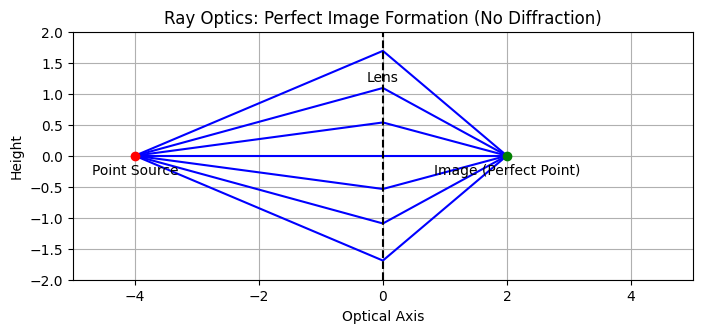
\includegraphics[width=0.45\textwidth]{../images/ray_optics_perfect_focus.png}
    \caption{Ray optics simulation of perfect image formation through a convex lens.}
    \label{fig:ray-focus}
\end{figure}

\subsubsection{Wave Optics Simulation}
Wave optics was then used to evaluate the same configuration. Modeling the lens aperture as a circular pupil,
the propagated field formed an Airy disk pattern due to diffraction. As shown in Figure~\ref{fig:wave-diffraction},
the intensity distribution exhibits a central bright lobe surrounded by concentric rings (although the intensity drops too low for them to be seen beyond the 2nd ring), a clear manifestation of the point
spread function (PSF). The 2D image and the horizontal cross-section intensity profile both highlight this effect.

\begin{figure}[H]
    \centering
    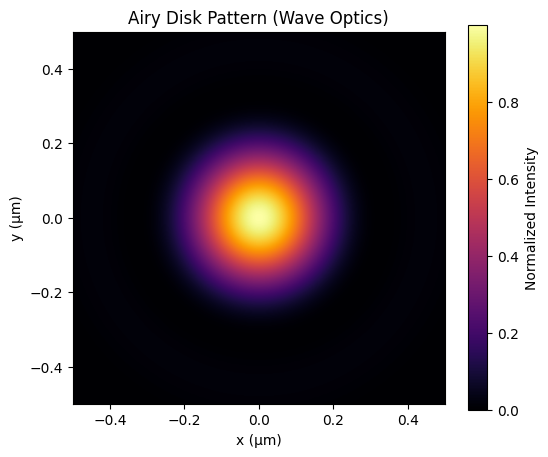
\includegraphics[width=0.45\textwidth]{../images/wave_optics_airy_disk.png}
    \caption{Wave optics simulation showing the Airy disk resulting from a circular aperture.}
    \label{fig:wave-diffraction}
\end{figure}

\subsection{Scenario 2: Aberrations in High-Aperture Lenses}

\subsubsection{Ray Optics Simulation}

In the second setup, an off-axis point source was imaged using a spherical lens with a high numerical aperture.
In the ray-based simulation (Figure~\ref{fig:ray-aberration}), rays that entered the lens at higher angles failed to converge at the same point as the central rays. This introduced spherical aberration,
resulting in a loss of resolution. The simulation captures the deviation of marginal rays and the mismatch at the focal region quite well.

\begin{figure}[H]
    \centering
    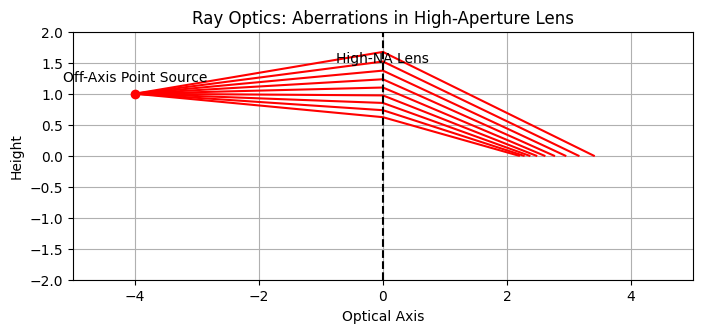
\includegraphics[width=0.45\textwidth]{../images/ray_optics_aberration.png}
    \caption{Ray optics simulation of aberration effects in high-aperture lens systems.}
    \label{fig:ray-aberration}
\end{figure}

\subsubsection{Wave Optics Simulation}

Wave optics simulation was then used to investigate the same aberrated system.
As shown in Figure~\ref{fig:wave-aberration}, the resulting PSF is significantly distorted compared to the ideal Airy disk shown before.
Off-axis field contributions interfere destructively and constructively across the aperture, leading to intensity shifts
and asymmetric blurring. These effects align well with 0ur theoretical expectations for aberration-induced phase errors.

\begin{figure}[H]
    \centering
    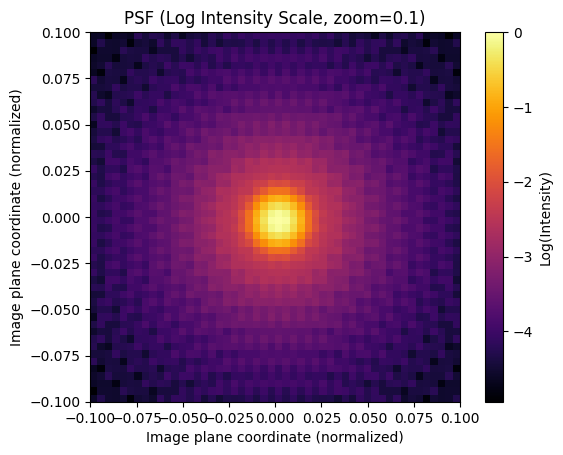
\includegraphics[width=0.45\textwidth]{../images/wave_optics_aberration.png}
    \caption{Wave optics simulation showing PSF distortion and off-axis interference patterns due to lens aberrations.}
    \label{fig:wave-aberration}
\end{figure}

\subsection{Discussion}

The results of the simulations reinforce the theoretical predictions we established earlier.
In the diffraction-limited imaging scenario, ray optics successfully predicted the focal point, yet failed to capture
the spreading of light caused by diffraction. Wave optics, in contrast, clearly visualised the Airy disk and the limited imaging resolution.

In the second scenario, ray optics again captured the geometric origin of aberrations, including the misalignment of
off-axis rays. However, the wave optics model revealed additional information, such as interference-induced
asymmetries and intensity deviations, which are important to understanding how aberrations degrade contrast and quality.

Ultimately, ray optics provided useful qualitative insights and remains valuable for initial optical design and intuition.
However, wave optics offered a more complete and physically accurate representation of the optical systems, especially
when modeling phenomena such as diffraction and aberrations. This validates the necessity of employing wave-based models
in high-resolution or precision imaging applications.
\end{multicols}